\chapter{System Design}

\section{Architectural Pattern}
\label{sec:arch-pattern}


The architecture of the platform is organized according to a layered approach composed of Presentation, Domain, and Data layers, leveraging the Model-View-ViewModel (MVVM) pattern combined with a Unidirectional Data Flow (UDF). This architectural decision was made to ensure a clear separation of concerns across the application. Rather than concentrating UI logic, business rules, and persistence concerns in the same components, the project distributes responsibilities across dedicated layers, improving readability, maintainability, and the capacity to evolve the system incrementally.

To manage dynamic data and user interactions, the platform adopts a UDF pattern, which formalizes the cycle of state production and consumption. In this model, state holders, typically implemented as ViewModel instances, act as the source of truth, transforming application data into an immutable UI state that the view layer observes. This interaction follows a well-defined cycle: the UI layer consumes and renders the state, while user events are propagated upward to the ViewModel, which processes the logic and initiates any necessary state mutations. By enforcing this flow, the UI is liberated from business logic responsibilities, allowing it to remain focused exclusively on display concerns, thereby enhancing testability, data consistency, and architectural maintainability.\cite{udf}

Several architecture patterns for mobile development were considered, namely Model-View-Controller (MVC), Model-View-Presenter (MVP), and Model-View-ViewModel (MVVM). All pursue the separation of user interface concerns from application logic but differ in how presentation coordination is organized. MVC structures the application around a controller that coordinates updates between the view and the model, which can make the UI flow tightly driven by imperative interactions. MVP improves on this by introducing a presenter that mediates between the view and the model, but the view remains tightly coupled to the presenter, and the pattern can add an extra mediation layer without fully leveraging state-based UI updates. MVVM, by contrast, exposes presentation state through a ViewModel and uses data binding, allowing the view to render observable state directly. This supports clearer decoupling, easier unit testing of presentation logic, and a more natural fit with the declarative UI approach adopted in this project.\cite{mvvm}.

 When paired with UDF, MVVM becomes significantly more robust, as UDF provides the specific guidelines needed to handle state mutations consistently across multiple screens. For this reason, MVVM with UDF was preferred over MVC and MVP, as it provides a superior foundation for incremental development, complex state management, and long-term maintainability \cite{mvvm, udf}.

The Figure \ref{fig:architecture} represents the project's architecture and some technologies that will be used, decided after the gathering of requirements.

\begin{figure}[h]
	\centering
	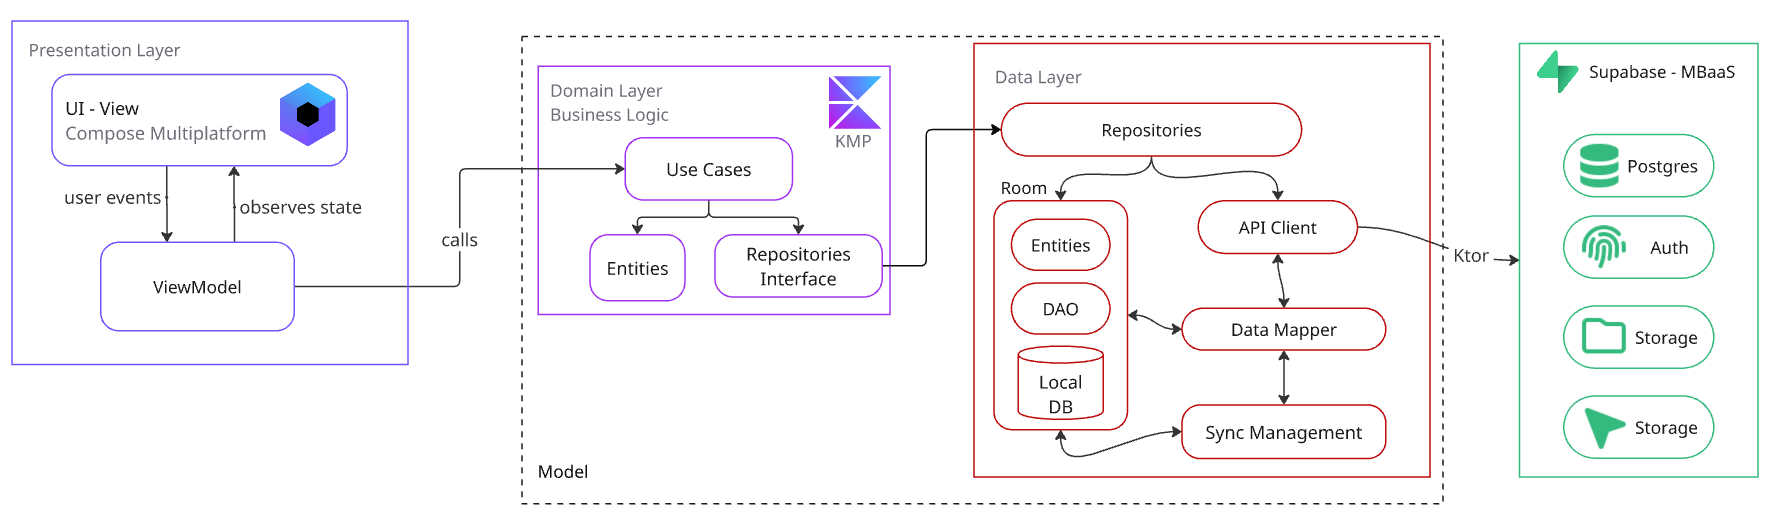
\includegraphics[width=1\textwidth]{figs/architectureDiagram}
	\caption{Architecture Diagram of the Multiplatform Application}
	\label{fig:architecture}
\end{figure}

The Presentation layer contains the composables that render the interface and the ViewModels that hold the observable state for each screen. The UI reacts to state changes exposed by the ViewModel, while user interactions, such as submitting a game, selecting a court, or applying filters, are propagated upward as events rather than triggering direct data manipulation from the View itself. This unidirectional data flow supports predictable behaviour, since each state transition can be traced from user action to ViewModel processing and then to the resulting update in the interface.

The Domain layer, that can be optional\cite{guideArchitecture}, concentrates the application-specific rules that define the behaviour of the platform. In this layer, Use Cases coordinate operations such as creating a game, checking court availability, joining a match, or updating player information, while remaining independent from the details of the database or external services, creating abstracting the Data Layer's repositories. This indirection is important because it allows the system to evolve without rewriting business rules whenever the persistence strategy or backend provider changes.

The Data layer is responsible for implementing the concrete data access strategy. It encapsulates repositories, local persistence, remote communication, and data mapping, so that the rest of the application works with domain models instead of database entities or network DTOs (data transfer objects). In practice, this means the ViewModel does not communicate directly with Room or Supabase, instead, it calls a repository which decides whether information should come from the local database, the remote backend, or a synchronisation routine.

This architecture was also selected because it aligns well with the acceptance test-driven development strategy adopted in the project. Because domain logic is separated from the user interface, acceptance criteria and behavioural tests can target the application rules directly, while the data layer can be substituted with test doubles or fakes during validation. As a result, the project gains improved testability, more stable incremental development, and better traceability between user stories and implementation decisions.

For this dissertation, the architectural pattern is therefore not merely a technical preference but a structural decision that supports the objectives of the system. It provides a stable foundation for the multiplatform implementation, simplifies the integration of offline-first behaviour and backend synchronisation, and creates a codebase that is easier to understand, test, and extend in a controlled manner.


\section{Cross-Platform Strategy}
\label{sec:arch-crossplatform}

The platform adopts a cross-platform strategy to maximize mobile reach while controlling development and maintenance effort, being one of the non-functional requirement, the platform needs to be available for Android and iOS.
Rather than developing two fully independent native applications, the project uses Kotlin Multiplatform( KMP )to share the core application logic across platforms. This approach allows the implementation of business rules, data handling, networking, validation, and synchronization-related code in a single codebase, while still preserving native capabilities where needed. For the user interface, Compose Multiplatform is used so that screens can also be shared, reducing duplication and improving consistency across platforms. Since the comparative analysis was already addressed in the Section \ref{sec:sota-mobile}, this one focuses on how the selected strategy was applied in the system design rather than revisiting the full technology comparison.

The main architectural principle adopted was separation between shared logic and platform-specific integration. The shared codebase contains the application’s core behaviour, including domain logic, data access, networking, state handling, and reusable UI components, while the Android and iOS modules act as thin platform entry points that configure the runtime and connect the shared application to each operating system. This structure reduces code duplication and ensures that changes in common functionality are propagated consistently across both platforms.

\subsection{Project Structure}

The project is organized around three main areas: the \texttt{composeApp module}, the \texttt{androidApp module}, and the \texttt{iosApp module}. The \texttt{composeApp module} is where the share code goes, most of the application logic is implemented, including the composable screens, dependency injection setup, and abstractions used by both platforms. The \texttt{Android module} is responsible for launching the shared UI inside an Android activity and handling Android-specific services such as permissions, image acquisition, and intent-based navigation. The \texttt{iOS module} is implemented in Swift and provides the application entry point, lifecycle handling, and integration with the shared Compose-based interface.

This modular structure supports maintainability because each platform layer remains small and focused. It also improves portability, since most feature changes can be implemented once in the shared layer instead of being duplicated in two independent native applications. At the same time, the design leaves room for platform-specific adaptations whenever the user experience or operating-system integration requires it.

\dirtree{%
	.1 root.
	.2 androidApp.
	.3 src.
	.4 main.
	.5 kotlin.
	.6 {com.theplayground}.
	.3 build.gradle.kts.
	.2 composeApp.
	.3 src.
	.4 androidMain.
	.5 kotlin.
	.6 {com.theplayground.shared}.
	.5 res.
	.4 commonMain.
	.5 kotlin.
	.6 {com.theplayground.shared}.
	.5 composeResources.
	.4 commonTest.
	.5 kotlin.
	.6 {com.theplayground.shared}.
	.5 resources.
	.4 iosMain.
	.5 kotlin.
	.6 {com.theplayground.shared}.
	.3 build.gradle.kts.
	.2 iosApp.
	.3 Configuration.
	.3 iosApp.
}   


Kotlin Multiplatform organises shared and platform-specific code through a hierarchy of source sets. The \texttt{commonMain} source set contains all code that is fully shared across platforms, including domain logic, data models, repository abstractions, networking, state management, and reusable UI components. This code is compiled for every target and cannot reference any platform-specific API directly.

Platform-specific source sets, \texttt{androidMain} and \texttt{iosMain}, complement the common layer by providing implementations that depend on Android or iOS APIs respectively. These source sets are only compiled for their corresponding target, which means they can freely reference platform SDKs while remaining invisible to the other platform. The Kotlin compiler resolves the correct source set at compile time, so the rest of the application always interacts with the common abstraction regardless of the underlying platform.

This structure enforces a clean boundary between shared behaviour and platform integration. Most of the application lives in \texttt{commonMain}, while \texttt{androidMain} and \texttt{iosMain} remain thin layers that only exist where the operating system requires a concrete, platform-native integration.

\subsection{Platform Abstractions with Expect/Actual}

Bridging shared code with platform-specific behaviour is one of the central challenges in any Kotlin Multiplatform project. 
Two complementary strategies were adopted depending on the nature of the integration required: the Kotlin \texttt{expect}/\texttt{actual} mechanism and interface-based dependency injection (DI). 
The choice between them is not arbitrary, each strategy has distinct characteristics that make it appropriate for different kinds of platform integration.

\subsubsection{Expect/Actual}

The \texttt{expect}/\texttt{actual} mechanism is a compiler-level construct built into Kotlin Multiplatform.
A declaration marked \texttt{expect} in \texttt{commonMain} signals that a platform-specific counterpart, marked \texttt{actual}, must be provided in every configured target source set.
The compiler enforces this contract at build time, eliminating the risk of a missing implementation surfacing at runtime. 
Crucially, resolution happens entirely at compile time: the compiled Android binary contains the Android implementation and the iOS binary contains the iOS one. 
There is no runtime polymorphism involved.

This strategy is best suited for two scenarios: when the abstraction itself cannot be expressed without platform-specific knowledge, and when the type requires platform-specific arguments at construction time that cannot be provided by a dependency injection container.
In this project it was applied to these cases: \textbf{secure storage}, \textbf{database initialisation}, and \textbf{the image picker}.

Secure storage is a representative example. 
The common declaration exposes a simple key-value API:

\begin{lstlisting}[language=java, caption={SecureStorage expect declaration (commonMain)}]
	expect class SecureStorage(context: Any? = null) {
		fun save(key: String, value: String)
		fun read(key: String): String?
		fun delete(key: String)
		fun clear(keys: List<String>)
	}
\end{lstlisting}

The reason \texttt{expect}/\texttt{actual} is required here, rather than an interface, is that the class itself is fundamentally platform-specific.
The Android actual requires an Android \texttt{Context} object to be passed at construction in order to access \texttt{SharedPreferences} and the \texttt{AndroidKeyStore}.
This argument cannot be expressed in common Kotlin nor provided transparently by a DI container operating at the common level, it must be supplied explicitly by the Android entry point.
There is simply no shared implementation possible and the class cannot even be constructed without knowing the platform.
The \texttt{expect} constructor accepts an \texttt{Any?} parameter, which functions as a platform-agnostic handle. This is necessary because the common module cannot reference the Android \texttt{Context} type directly. At runtime, the Android implementation performs a checked cast of this dependency to access system services, while the iOS implementation ignores the parameter, as the Apple Security framework does not require a host context for Keychain access.

On Android, the actual implementation encrypts values with AES-256-GCM using a key stored in the \texttt{AndroidKeyStore} and persists the resulting ciphertext in \texttt{SharedPreferences}:

\begin{lstlisting}[language=java, caption={SecureStorage actual — Android save (androidMain)}]
	actual fun save(key: String, value: String) {
		val encrypted = encrypt(alias = key, plaintext = value)
		prefs.edit().putString(key, encrypted).apply()
	}
\end{lstlisting}

On iOS, the same contract is satisfied through direct Keychain access via the Security framework.
In both cases the session management layer in \texttt{commonMain} interacts solely with the \texttt{expect} declaration and remains entirely unaware of the underlying storage mechanism.
Database initialisation follows the same reasoning: the SQLDelight driver requires a \texttt{Context} on Android and a different native driver on iOS, leaving no common ground for a shared implementation.

The image picker follows a similar pattern but introduces a deliberate hybrid approach.
The \texttt{expect}/\texttt{actual} mechanism is necessary because of a constraint specific to Android. Launching the camera or gallery requires registering an \texttt{ActivityResultLauncher}\footnote{\texttt{ActivityResultLauncher} must be registered before or during the \texttt{onCreate} phase of the Android lifecycle. Because the API throws an \texttt{IllegalStateException} if initialized after the host component has started, the registration cannot be deferred to a shared ViewModel or a lazy-loaded component that operates during the \texttt{resumed} state.} during the host component's initialization phase. This registration cannot be deferred or triggered lazily from shared code.
Consequently, the Android actual exposes an \texttt{initialize} method that the Android Activity calls at startup to register those launchers, passing them as callbacks into the shared singleton.
On iOS this method is a no-op, because iOS imposes no such constraint since a \texttt{UIViewController} can be presented at any point, so the iOS actual presents the picker directly when the coroutine is invoked.

The hybrid aspect is that the \texttt{expect} declaration is backed by a singleton \texttt{object} rather than a class, reflecting the fact that the picker is a stateful coordinator bound to the UI lifecycle rather than an instantiated service, and the shared layer interacts with it through a common \texttt{ImagePickerContract} interface.
This preserves substitutability for testing even though the underlying resolution is compiler-driven.
The shared presentation layer remains uniform, it always calls \texttt{ImagePicker.pickImageFromGallery()} or \texttt{ImagePicker.takePhotoWithCamera()}, while each platform accommodates its own callback model internally.

The \texttt{ImagePickerContract} interface wrapper is not required for correct cross-platform behaviour, the \texttt{expect}/\texttt{actual} singleton alone would suffice, but it is introduced to allow the picker to be substituted with a fake implementation in unit tests, where no real camera or gallery is available.

\subsubsection{Interface-Based Injection}

For integrations where the abstraction can be expressed entirely in common Kotlin, interface-based dependency injection is preferable to \texttt{expect}/\texttt{actual}.
Rather than relying on the compiler to swap implementations, the shared layer depends on an interface and the correct concrete class is provided at runtime by the platform-specific dependency injection module.
This approach naturally supports substitution for testing and allows the DI container to own the full lifecycle of the service.

The key distinction from the \texttt{expect}/\texttt{actual} cases is constructibility. 
\texttt{ConnectivityMonitor} and the location service do not require a platform-specific argument to be passed by the caller, the DI container, which is configured per platform, already has access to the Android \texttt{Context} and can supply it when building the object graph.
The interface itself contains nothing platform-specific:

\begin{lstlisting}[language=java, caption={ConnectivityMonitor interface (commonMain)}]
	interface ConnectivityMonitor {
		val isOnline: StateFlow<Boolean>
		fun dispose() {}
	}
\end{lstlisting}

Because \texttt{ConnectivityMonitor} is a long-lived service that registers OS callbacks and holds system resources, it is also appropriate for the DI container to manage its lifecycle, calling \texttt{dispose()} when the application is shutting down. 
This kind of lifecycle ownership is natural with interface injection but awkward with \texttt{expect}/\texttt{actual}, where the compiler resolves the type but imposes no lifecycle model.

The Android implementation registers a \texttt{ConnectivityManager.NetworkCallback} and maintains a set of active internet-capable networks to derive online status.
The iOS implementation uses the \texttt{Network} framework's \texttt{nw\_path\_monitor} API.
The contrast between the two platform DI modules illustrates precisely why this strategy is viable: on Android, \texttt{androidContext()} is passed by the container, confirming that the \texttt{Context} dependency is resolved without caller involvement while on iOS, the constructor requires no platform argument at all.

\begin{lstlisting}[language=java, caption={Platform DI modules — relevant bindings}]
	// androidMain
	val platformModule = module {
		single<ConnectivityMonitor> { AndroidConnectivityMonitor(androidContext()) }
		single<NativeLocationProvider> { AndroidLocationProvider(androidContext()) }
	}
	
	// iosMain
	val platformModule = module {
		single<ConnectivityMonitor> { IosConnectivityMonitor() }
		single<NativeLocationProvider> { IosLocationProvider() }
	}
\end{lstlisting}

In both cases, the rest of the application references only the \texttt{ConnectivityMonitor} interface, remaining entirely decoupled from the platform-specific implementations registered in each module.

\subsubsection{Choosing Between the Two Strategies}

The two strategies are not interchangeable and the decision follows a clear heuristic. 
If the type itself is platform-specific, because it requires a platform-native constructor argument that cannot be supplied by the DI container, or because no shared description of it is possible in common Kotlin, \texttt{expect}/\texttt{actual} is the appropriate tool, as the compiler must select the implementation. 
If only the implementation is platform-specific while the abstraction can be expressed in common Kotlin and the DI container can supply any platform dependencies during object construction, interface injection is preferable, as it enables runtime substitution and natural lifecycle management.
Together, the two mechanisms cover the full range of platform integration needs without compromising the architectural boundary between the shared module and the platform entry points.

\section{Frontend Architecture}
\label{sec:arch-frontend}


\subsection{Navigation Architecture}
\label{subsec:nav-architecture}

The application's navigation was designed to balance rapid accessibility with systemic simplicity. Following a comparative analysis of different options, a bottom navigation bar was implemented as the primary global mechanism. To ensure alignment with \textbf{Material Design 3 (MD3)} guidelines \footnote{https://m3.material.io/components/navigation-bar/guidelines}, which recommend between three and five primary destinations, the architecture utilizes four core paths: Home, Courts List, Games List, and Players List.

The following sections detail the navigation flows specific to each functional module.

\subsubsection{Courts Module}
The Courts module (Figure \ref{fig:nav-diag-courts}) follows a hierarchical drill-down pattern. Starting from the navigation bar or other high-level "root" screens, users transition to the Courts List and subsequently to the Court Details. A key design objective was maintaining a "shallow" navigation stack; by utilizing internal tabs within the Details view, users can pivot between various facility features without performing multiple "Back" actions. This ensures that the court context remains persistent while the user explores games, players, or rankings.

\begin{figure}[h]
	\centering
	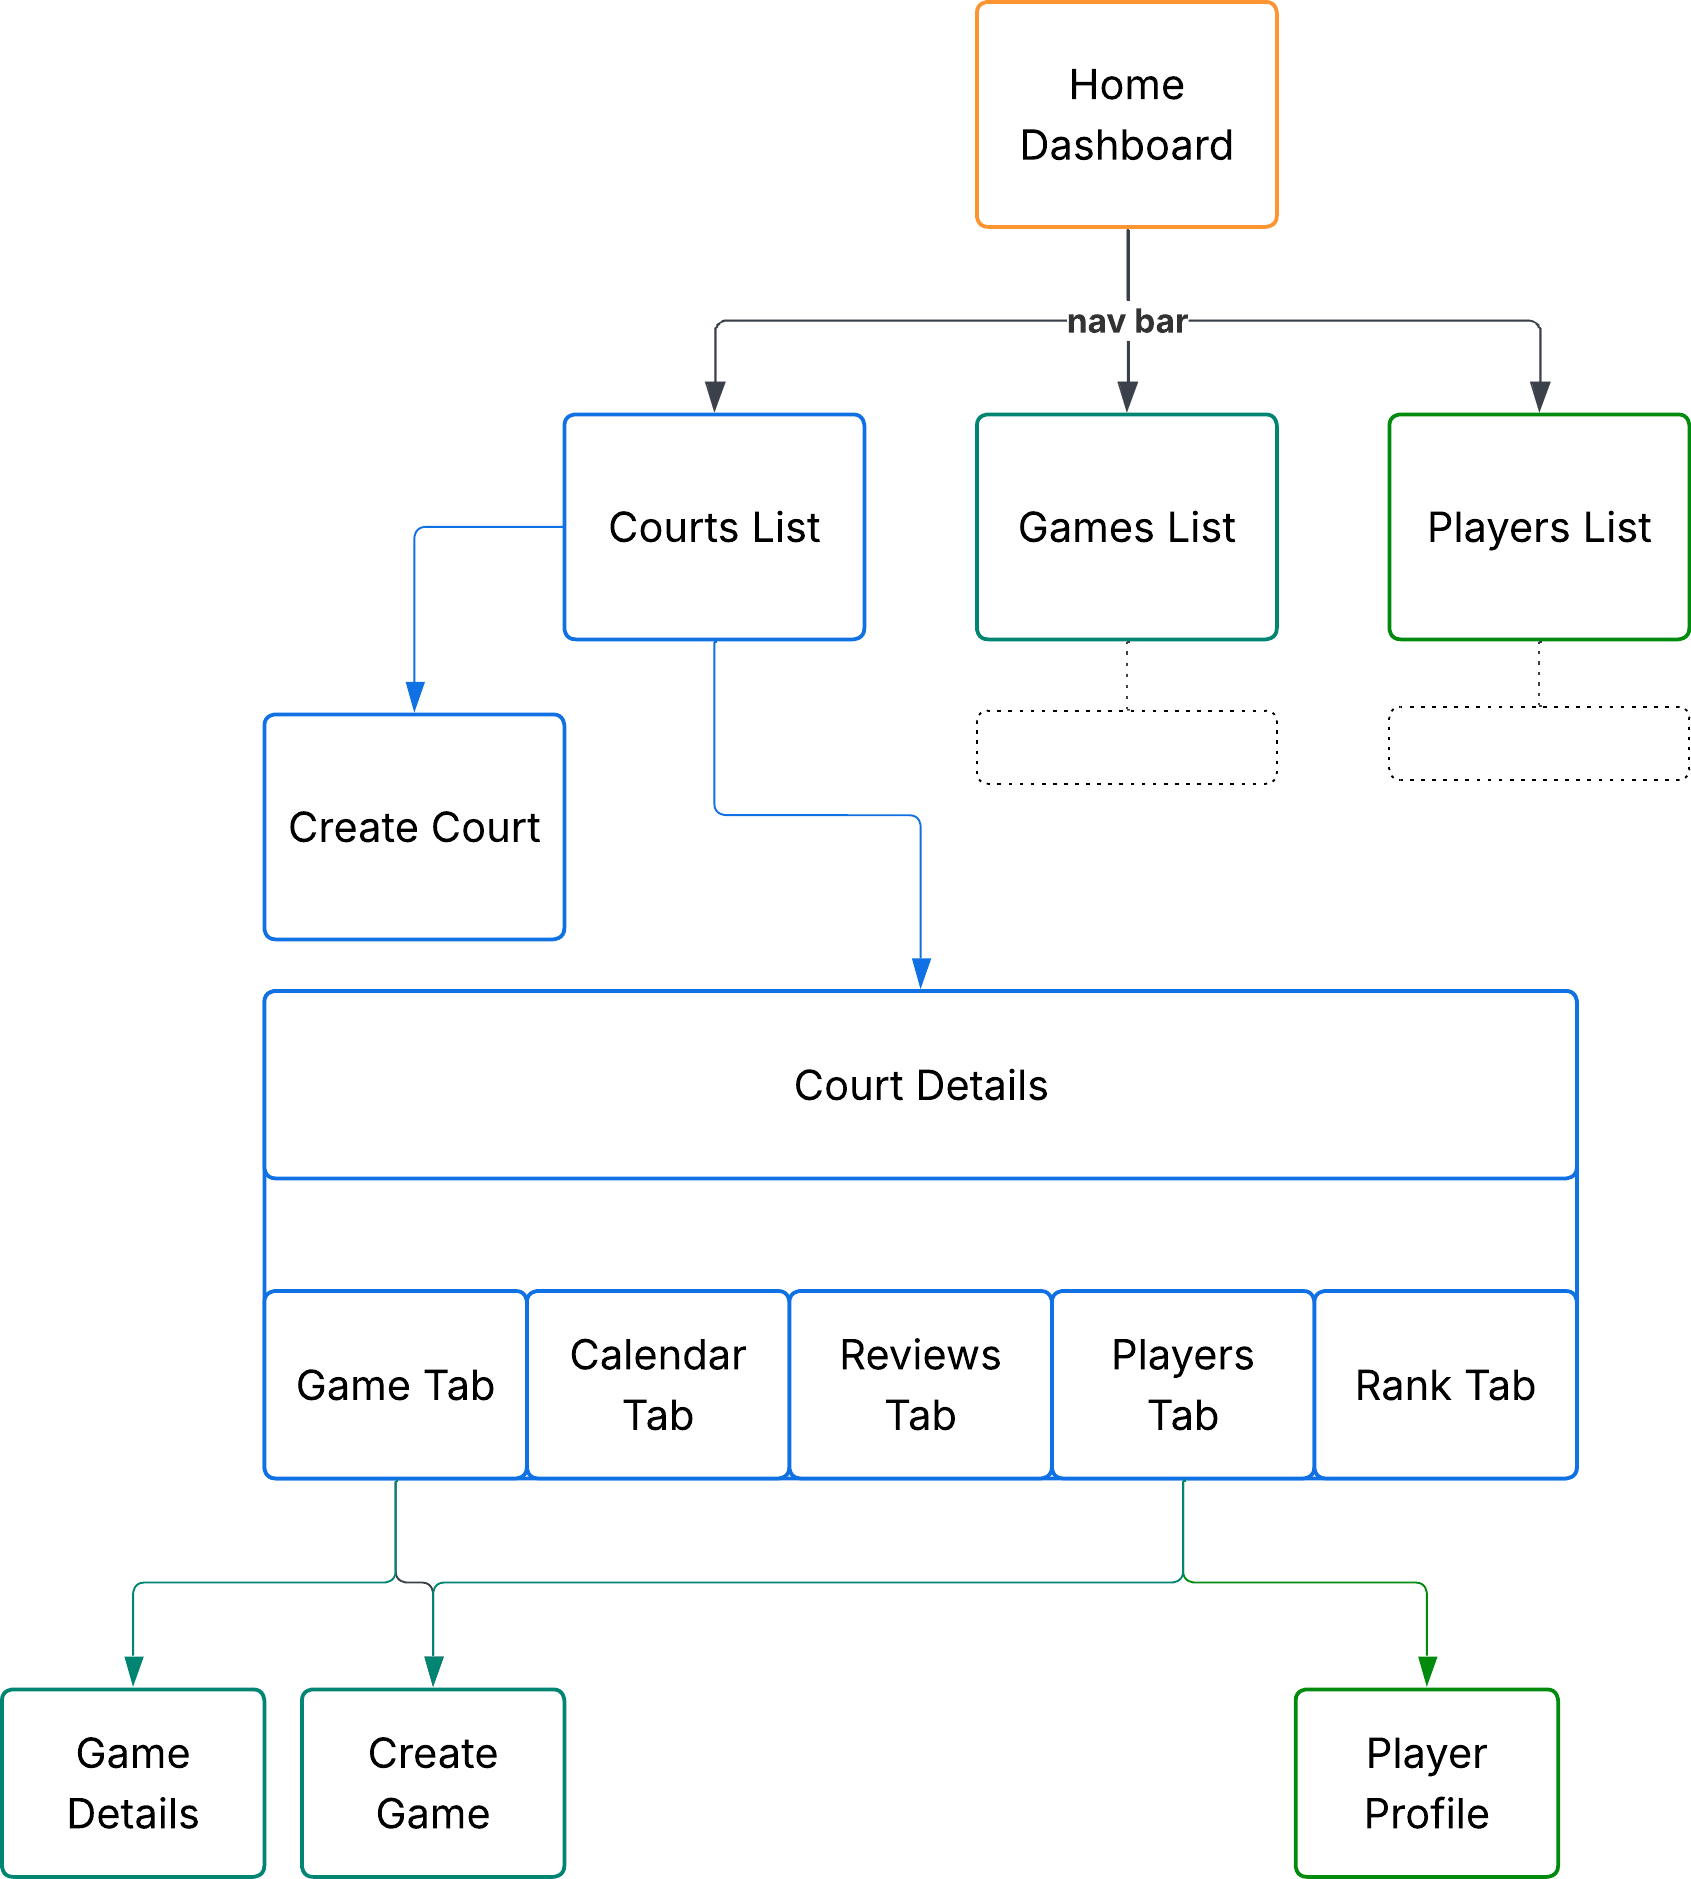
\includegraphics[width=0.7\textwidth]{figs/navigation-diagram/courts.png}
	\caption{Navigation Diagram - Courts Module Flow}
	\label{fig:nav-diag-courts}
\end{figure}

\subsubsection{Games Module}
Consistent with the established navigation logic, the Games module allows users to access the Games List via the global navigation bar. As illustrated in Figure \ref{fig:nav-diag-games}, selecting a specific match navigates the user to the Game Details view. This flow is designed for rapid discovery, allowing users to move from the global overview to specific match management in a two-step sequence.

\begin{figure}[h]
	\centering
	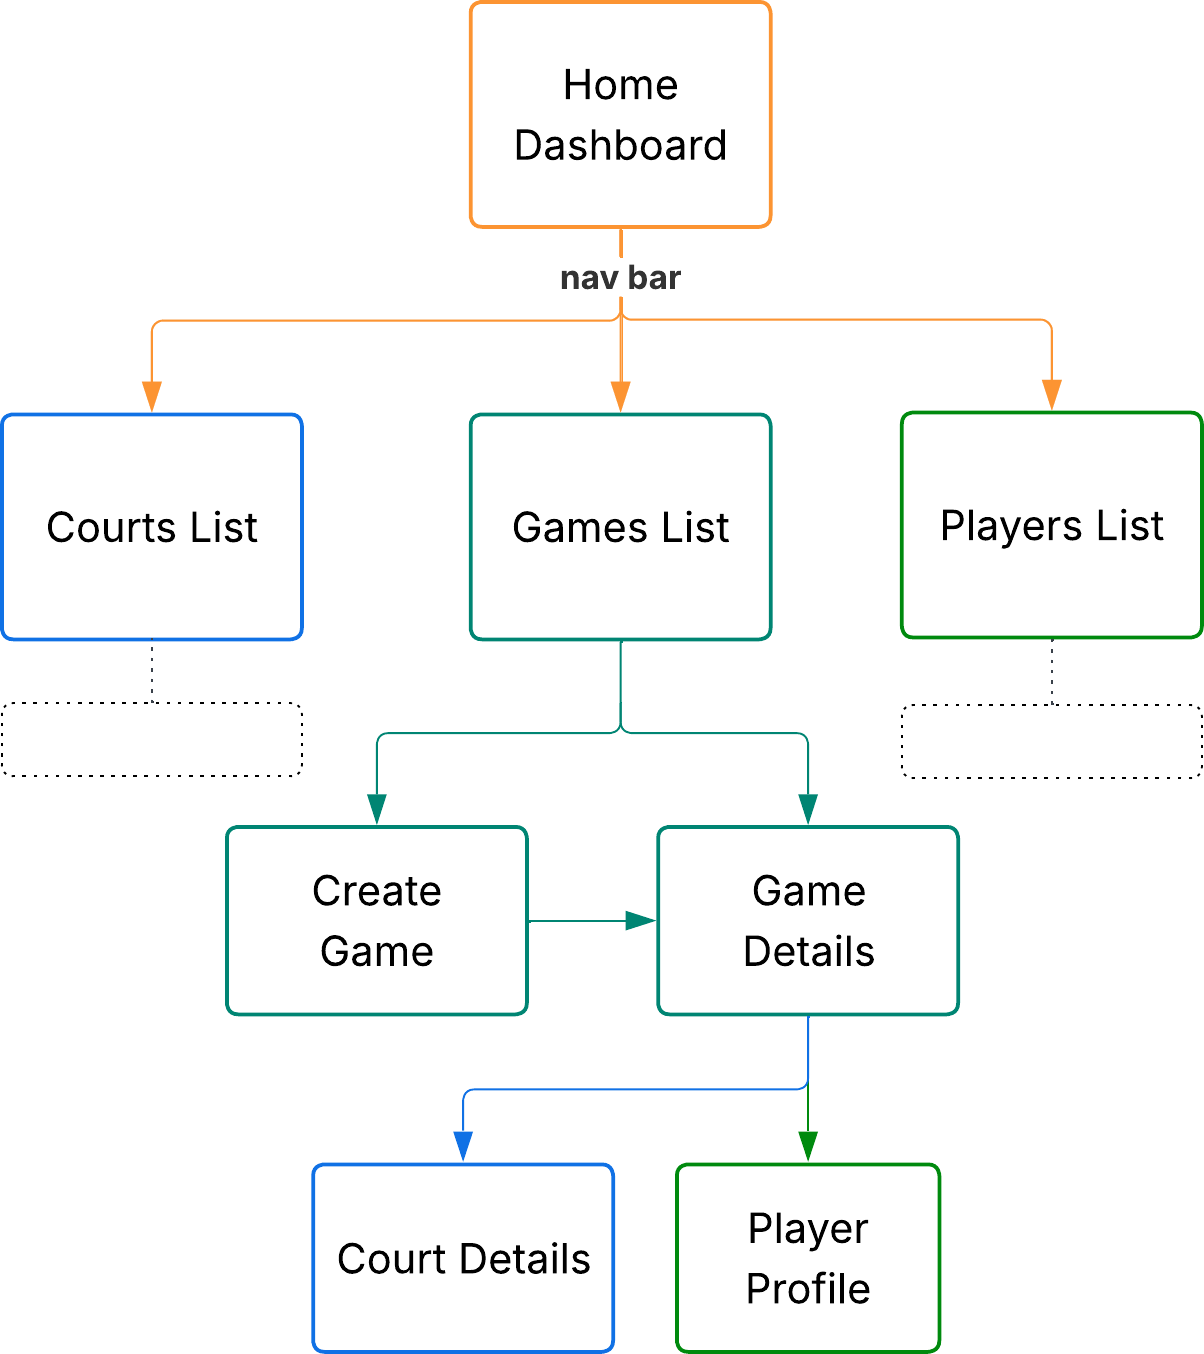
\includegraphics[width=0.7\textwidth]{figs/navigation-diagram/games.png}
	\caption{Navigation Diagram - Games Module Flow}
	\label{fig:nav-diag-games}
\end{figure}

\subsubsection{Players Module}
The Players module provides dual entry points to support both social discovery and personal identity management. Users can access their personal profile directly from the Home dashboard, while the global navigation bar provides access to the broader Players List. As shown in Figure \ref{fig:nav-diag-players}, selecting a user from the list navigates to their specific Player Profile. 

The profile view utilizes the same internal tab logic as the Court Details to maintain a consistent mental model across the application. Furthermore, the Home dashboard integrates a "Notifications Hub" allow users to bypass standard list views and navigate directly to relevant Game Details or Player Profiles in response to invites, requests, match updates, and other notifications.

\begin{figure}[h]
	\centering
	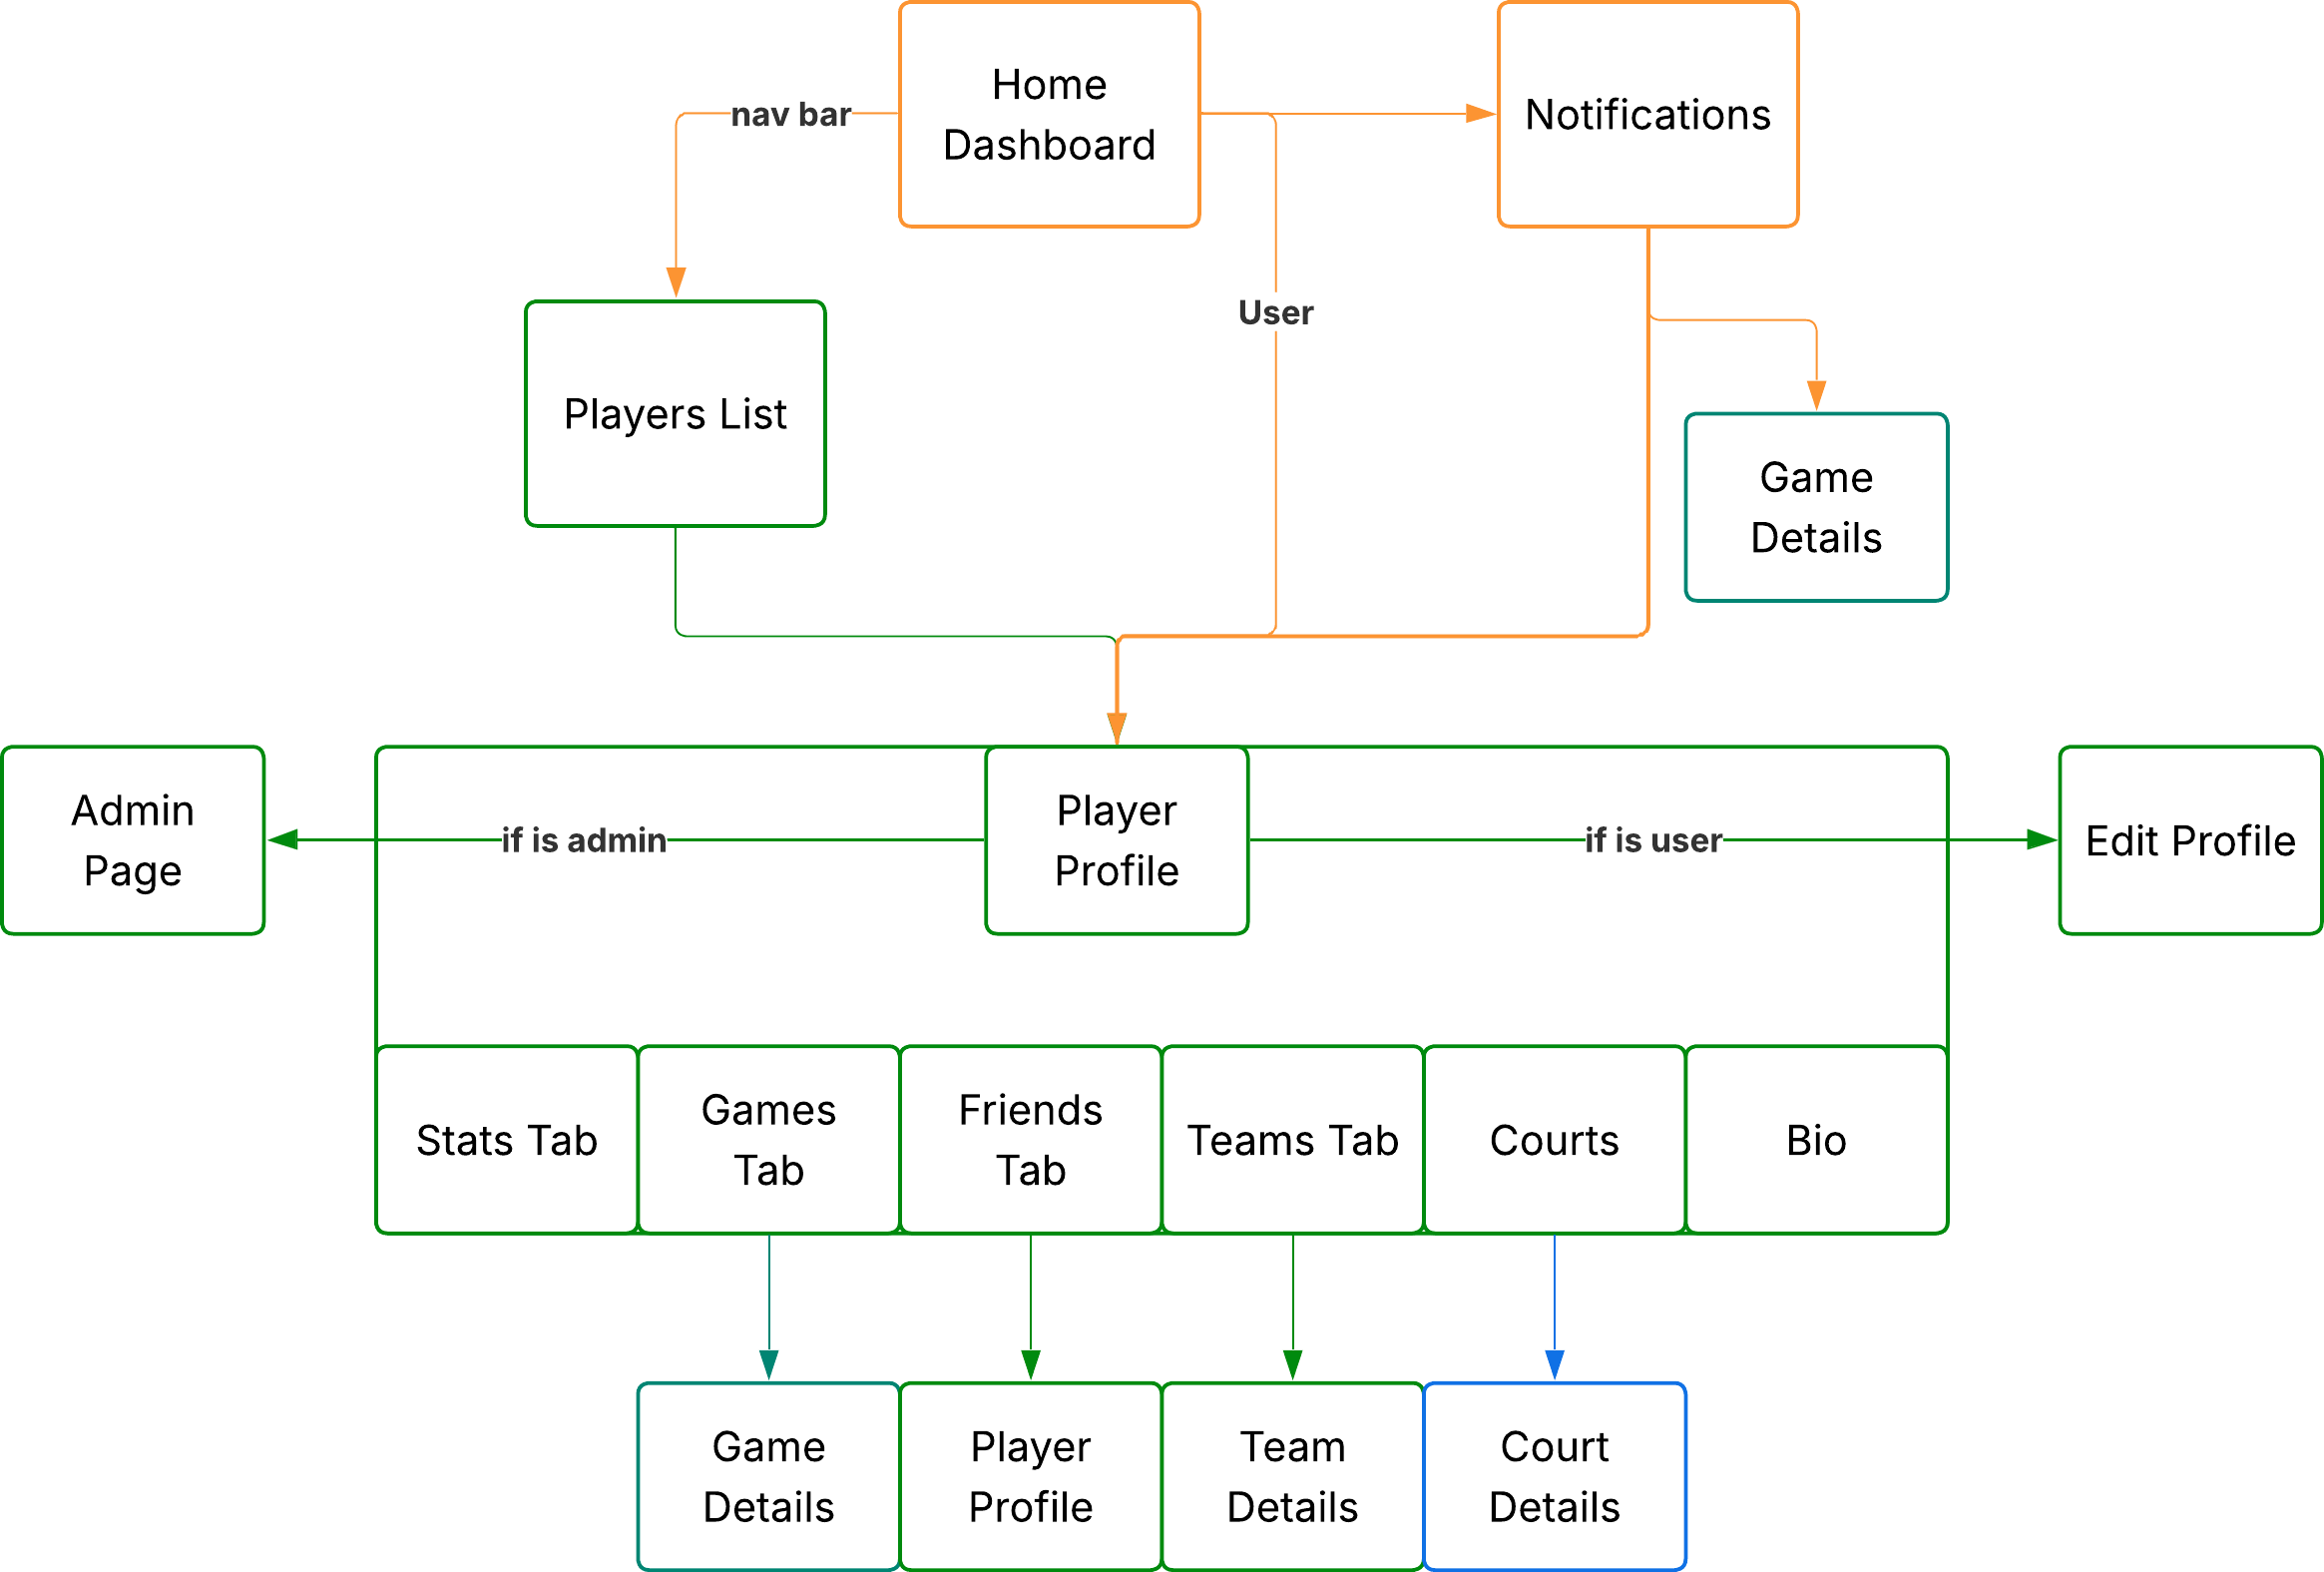
\includegraphics[width=0.7\textwidth]{figs/navigation-diagram/players.png}
	\caption{Navigation Diagram - Players Module Flow}
	\label{fig:nav-diag-players}
\end{figure}



\section{Backend Architecture }

The backend architecture is design to provide a robust, scalable  and secure environment for processing and storing user data. 


\subsection{Supabase}
\label{sec:arch-supabase}

Following the evaluation of Mobile Backend as a Service (MBaaS) options in Section \ref{subsec:mbaas}, Supabase was selected due to its comprehensive service suite, generous resource quotas, and the absence of vendor lock-in. The project utilized a dual-environment configuration:

\begin{itemize}
	\item \textbf{Supabase CLI:} A local development environment running via Docker. This enabled rapid iteration, offline development, and testing without consuming cloud-environment quotas. The local instance provides a management dashboard accessible via \textit{localhost}.
	\item \textbf{Supabase Cloud:} The production-grade environment. The cloud project was linked to the local CLI to allow for seamless synchronization of schemas and configurations.
\end{itemize}

The CLI initializes a dedicated project directory containing configuration files and a \texttt{migrations} folder. This migrations directory contains the SQL scripts required to evolve the database schema. These scripts ensure that the database remains consistent across different development machines and can be synchronized with the cloud environment via the terminal.

Supabase provides several integrated services utilized in this project:
\begin{itemize}
	\item \textbf{Authentication:} Identity management and session handling.
	\item \textbf{PostgreSQL Database:} Relational data storage with Row-Level Security (RLS).
	\item \textbf{Storage:} object storage for media assets.
	\item \textbf{Realtime:} Synchronization of data changes via WebSockets.
\end{itemize}

The \texttt{SupabaseClient} is initialized as a singleton using the Koin dependency injection framework. As shown in Listing \ref{lst:supabase-init}, the client installs the required modules and manages the user session lifecycle automatically.

\begin{lstlisting}[language=java, caption={Supabase Client Initialization}, label={lst:supabase-init}]
	single {
		createSupabaseClient(supabaseUrl, supabaseKey) {
			install(Postgrest)
			install(Auth) {
				sessionManager = get<SupabaseSessionManager>()
				autoSaveToStorage = true
				autoLoadFromStorage = true
				alwaysAutoRefresh = true
			}
			install(Storage)
			install(Realtime)
		}
		.also { logger.e { "SupabaseClient created for environment: ${env.name}" } }
	}
\end{lstlisting}

Environment-specific configurations were managed via \texttt{.env} files. A notable challenge in the development phase involved the Android emulator's networking constraints. While iOS can access a local Supabase instance via \texttt{localhost}, Android emulators require the loopback address \texttt{10.0.2.2}. To resolve this, the \texttt{expect}/\texttt{actual} pattern described in Section \ref{sec:arch-crossplatform} was employed to provide the correct host URL based on the target platform.

\subsubsection{Authentication}

The platform utilizes email and password authentication. Upon registration, Supabase generates a unique UUID for the user and triggers a verification email to ensure address validity. To maintain high deliverability and professional branding, \textbf{Resend} was integrated as the SMTP provider for the \texttt{theplayground.pt} domain.

To mitigate brute-force attacks and resource abuse, a rate-limiting policy was implemented. This rule restricts users to five authentication attempts within a five-minute window per IP address. By exceeding this limit triggers a temporary block, reflected in the User Interface by a countdown timer. Once authenticated, the session is persisted locally until an explicit sign-out action is performed.

\subsubsection{Storage}

Media assets, including court imagery and user profile pictures, are managed via Supabase Storage buckets. The storage is structured into two primary buckets:
\begin{itemize}
	\item \textbf{Courts Bucket:} Organized hierarchically, where each directory is named after the court's UUID to prevent naming collisions.
	\item \textbf{Profiles Bucket:} Stores individual player images, identified by the user's unique \texttt{player\_uuid}.
\end{itemize}

\subsection{Database Schema Design}
\label{subsec:arch-schema}

\subsection{Realtime Subscriptions}
\label{subsec:arch-realtime}


\section{Local Data Layer}
\label{sec:arch-local-data}

In the Data layer, there are the repositories, as the guide mentions\cite{guideArchitecture} which will work with a local and an external data source. The local data source will be Room\cite{room} that is part of Android Jetpack suite, making a good option for this project, being an abstraction of SQLite database, that integrates naturally with flows and coroutines, providing a annotation-based API. Compare to SQLDelight, a considerable option, it has slight more boilerplate with entities and DAOs, and less control over raw SQL, making debugging complex queries harder. 

For the external data source it will be use the Supabase, an open source MBaaS with several services available that will help with the project, including PostgreSQL Database that can handle complex relationship connections while offering built-in real-time features for live updates. Besides that, it has authentication, storage, and server-side functions, however, lacks native push notifications and mobile analytic, which forces third-party tools integrations. Supabase can be self-hosted or use theirs services that has different pricing options, with the free tier being enough for this project, as it has a limit of 50,000 monthly active users. Comparing to others, it is not a "black box" being easy to debug and has less vendor lock-in, with a PostgresSQL database that can be run anywhere and can be exported.

Using Ktor to communicate with Supabase as it is standard and recommend HTTP client, with multiple examples from Google, Jetbrains and other communities using Ktor as example in Kotlin Multiplatform projects. Another good option would be the Supabase Kotlin Client, however, this would make the application dependable on Supabase and if later the MBaaS was to be replaced, it would be more complex to migrate. With this, a little more code needs to be developed with Ktor, than Supabase Kotlin Client, but ideal to not get vendor lock-in. As some feature of the platform will need to work while the user is off-line or with bad connection, the application will have a synchronization manager that will check what needs to be updated in the local database and resolve conflicts. Finally a data mapper to convert data from Supabase to the Room database is needed.



\section{Libraries and other tools}


\subsection{Maps Engine}

An important piece of this project is to have a map identifying the courts for the users to find and visualize. There are several tools and libraries for this, however the most compatible and cheap option is MapLibre Compose\footnote{https://maplibre.org/maplibre-compose/}. This is a Compose Multiplatform wrapper around the MapLibre\footnote{https://maplibre.org/} SDKs, an organization that provides open-source mapping libraries, which enables to render interactive maps. The MapLibre Compose will work in both Android and iOS, and it is possible to configure gestures, respond to a map click or long click, download off-line images and more other features.

A disadvantage of this library is that the community and support is still growing. An alternative would be Google Maps SDK\footnote{https://developers.google.com/maps/documentation/android-sdk/overview?section=start}, however it has vendor lock-in, with costs passing the 300 USD (US Dollar) trial credits. Besides that, it is not Kotlin Multiplatform native, needing a platform-specific implementation. Mapbox\footnote{https://www.mapbox.com/} would be another option, with a free tier and then priced, with no direct support to KMP.

MapLibre Compose is used as a Presentation Layer component, acting as the UI rendering engine responsible for visualizing geospatial data exposed by the ViewModel. It is decoupled from business logic and data access, ensuring that domain rules related to court management remain independent of the specific mapping technology. In contrast, the MapLibre SDK integrates with the Data Layer, handling the retrieval of map tiles from external MapLibre servers when users pan, zoom, or change location. It also implements caching strategies to store map assets locally for off-line use and manages map styling by fetching and applying the MapLibre style JSON, which defines layers, colours, and other visual properties.

\subsection{Notifications Engine}

To keep user's engagement, it is essential to have notifications, when they are in the application and when they have the application closed, so they get notified when someone has created a game in their favourite court. Supabase have a real-time feature that enables to create in-app notifications, however, when the application is closed there it is no communication between the Supabase backend and the client side. For push notifications, when the application is closed, there are different options. Google's Firebase has the Firebase Cloud Messaging (FCM)\footnote{https://firebase.google.com/docs/cloud-messaging} that can notify the application about available synchronizations, and send notification messages to single devices, to groups of devices, or to devices subscribed to topics, all this with no costs. Another option is OneSignal\footnote{https://onesignal.com/} that has multiple functionalities including sending notifications when the application is closed. OneSignal has some pricing options, but in the free tier, the push notifications are unlimited. For this project, OneSignal will be used, as the set-up is easier, as it handles user's tokens while in Firebase, it needs more code to handle that part.

OneSignal integrates with the Data Layer, which handles push notification functionality. When a user creates a game, for example, the application makes an API call to OneSignal to send a push notification to users. By isolating notification logic in the Data Layer, the architecture remains agnostic to the specific notification provider, allowing future migration to alternative services without impacting business logic.


\section{Offline-First and Synchronisation Strategy}
\label{sec:arch-offline}

\section{Security Design}
\label{sec:arch-security}

\section{CI/CD Pipeline}
\label{sec:arch-cicd}



